\scanpage{28}

% The list and the ruled sheet share one coordinate field. Coordinates reproduce
% the supplied image's relative positions, including the long blank lower part.
% The faint far-left trace has fading, indeterminate ends: the path represents
% the observed segment, not an asserted original endpoint or a named operation.
\noindent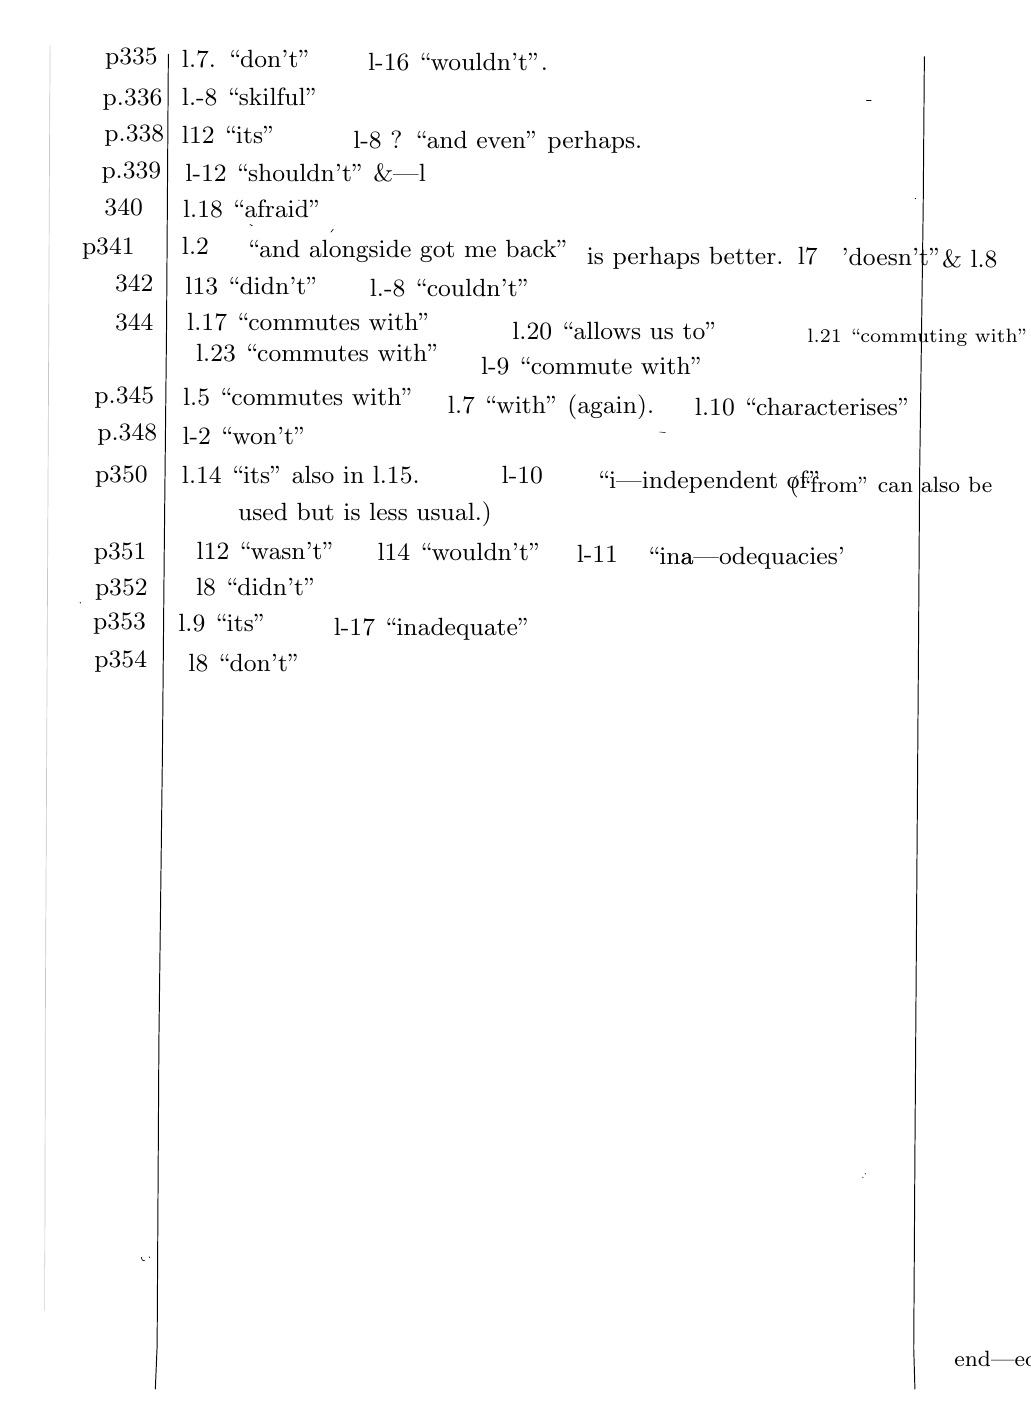
\begin{tikzpicture}[x=.0075cm,y=-.0075cm,line cap=round,line join=round]
\path[use as bounding box] (20,45) rectangle (1670,2348);
% BEGIN left_rule
\draw[line width=.35pt] (258,90)--(255,545)--(251,935)--(248,1270)--(242,1760)--(239,2275)--(236,2348);
% END left_rule
% BEGIN right_rule
\draw[line width=.35pt] (1537,94)--(1535,350)--(1529,800)--(1527,1100)--(1524,1520)--(1521,1950)--(1519,2280)--(1521,2348);
% END right_rule
% BEGIN faint_trace
\draw[black!22,line width=.25pt] (58,75)--(57,240)--(55,700)--(53,1100)--(50,1700)--(49,2140);\draw[black!12,line width=.25pt] (49,2140)--(49,2215);
% END faint_trace
% Prominent isolated marks, with no assigned punctuation or editorial function.
% BEGIN upper_right_dash
\draw[line width=.18pt] (1439,168)--(1447,168);
% END upper_right_dash
% BEGIN right_point
\fill (1522,334) circle[radius=1.0];
% END right_point
% BEGIN afraid_marks
\fill (479,337) circle[radius=1.1];\draw[line width=.24pt] (396,378)--(400,380);\draw[line width=.24pt] (533,391)--(537,386);
% END afraid_marks
% BEGIN again_mark
\draw[line width=.18pt] (1089,729)--(1099,730);
% END again_mark
% BEGIN left_352_point
\fill (109,1018) circle[radius=1.1];
% END left_352_point
% BEGIN lower_left_marks
\draw[line width=.24pt] (212,2125)--(214,2130)--(218,2131);\fill (226,2125) circle[radius=1.1];
% END lower_left_marks
% BEGIN lower_right_marks
\fill (1433,1990) circle[radius=1.0];\fill (1437,1984) circle[radius=1.0];
% END lower_right_marks

\begin{scope}[every node/.style={anchor=base west,inner sep=0pt,font=\fontsize{9}{11}\selectfont}]
\node at (150,108) {p335};
\node at (280,113) {l.7. ``don't''};
\node at (595,118) {l-16 ``wouldn't''.};

\node at (146,176) {p.336};
\node at (280,177) {l.-8 ``skilful''};

\node at (149,237) {p.338};
\node at (280,241) {l12 ``its''};
\node at (570,249) {l-8 ? ``and even'' perhaps.};

\node at (144,301) {p.339};
\node at (286,305) {l-12 ``shouldn't'' \deleted{\unsure{\&|l}}};

\node at (149,363) {340};
\node at (282,366) {l.18 ``afraid''};

\node at (111,429) {p341};
\node at (280,429) {l.2};
\node at (389,434) {``and alongside \uline{got me} back''};
\node at (965,445) {is perhaps better.};
\node at (1322,445) {l7};
\node at (1396,448) {'doesn't''};
\node at (1566,450) {\& l.8};

\node at (167,491) {342};
\node at (286,496) {l13 ``didn't''};
\node at (598,499) {l.-8 ``couldn't''};

\node at (167,557) {344};
\node at (289,558) {l.17 ``commutes with''};
\node at (839,573) {l.20 ``allows us to''};
\node[font=\fontsize{7}{9}\selectfont] at (1338,578) {l.21 ``commuting with''};

\node at (304,610) {l.23 ``commutes with''};
\node at (786,631) {l-9 ``commute with''};

\node at (132,680) {p.345};
\node at (282,685) {l.5 ``commutes with''};
\node at (730,697) {l.7 ``with'' (again).};
\node at (1148,701) {l.10 ``characterises''};

\node at (137,744) {p.348};
\node at (281,750) {l-2 ``won't''};

\node at (133,815) {p350};
\node at (280,817) {l.14 ``its'' also in l.15.};
\node at (821,817) {l-10};
\node at (981,824) {``\unsure{\uuline{i}|\uline{i}}ndependent of''};
\node[font=\fontsize{8}{10}\selectfont] at (1308,831) {(``from'' can also be};
\node at (375,879) {used but is less usual.)};

\node at (131,944) {p351};
\node at (305,944) {l12 ``wasn't''};
\node at (611,947) {l14 ``wouldn't''};
\node at (948,950) {l-11};
\node at (1066,953) {``in\tikz[baseline=(aold28A.base)]{\node[inner sep=0pt] (aold28A) {\deleted{\unsure{a|o}}};\node[anchor=base west,inner sep=0pt] at (aold28A.base west) {a};}dequacies'};

\node at (133,1006) {p352};
\node at (304,1005) {l8 ``didn't''};

\node at (130,1063) {p353};
\node at (274,1066) {l.9 ``its''};
\node at (537,1073) {l-17 ``inadequate''};

\node at (132,1127) {p354};
\node at (291,1134) {l8 ``don't''};
\end{scope}

% The cancelled marginal word is at the foot of the sheet, outside the right
% rule. The cancellation traverses the whole word; its buried n is not secure.
% BEGIN bottom_note
\node[anchor=base west,inner sep=0pt,font=\fontsize{8}{10}\selectfont] at (1587,2310) {\deleted{\unsure{end|ed}}};
% END bottom_note
\end{tikzpicture}

% archive sheet number: 27
